\textbf{3)} As reações paralelas de substituição nucleofílica bimolecular (\ce{Sn 2}) e eliminação bimolecular de formaldeído (\ce{Eco 2}) observadas entre o nitrato de metila (\ce{MeNO3}) e o íon hidróxido foram estudadas e são representadas com suas respectivas constantes de velocidade abaixo:

\begin{align*}
    \ce{MeNO3 + ^-OH &->[{k_{SN 2}}] CH3OH + NO3^-} \\
    \ce{MeNO3 + ^-OH &->[{k_{Eco 2}}] H2O + CH2O + NO2^-}
\end{align*}

Esse estudo experimental foi conduzido a temperatura e pressão constantes e em excesso de nitrato de metila, fornecendo os dados cinéticos a seguir. As reações também foram modeladas do ponto de vista teórico, fornecendo valores de energia relativos dos ``reagentes'' e dos estados de transição, conforme apresentado no diagrama a seguir.

\begin{figure}[H]
    \centering
    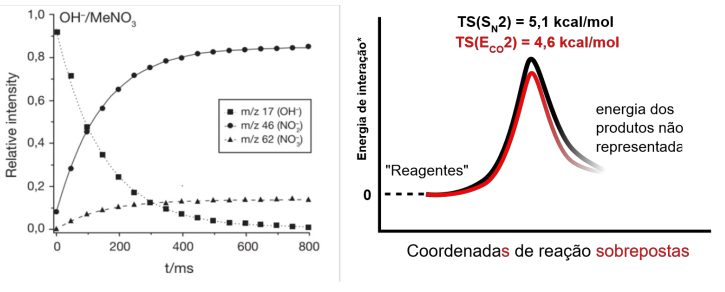
\includegraphics[width=\textwidth]{fig/diagramQ3}
\end{figure}

Considere que os dados teóricos fornecem a estrutura dos reagentes e dos estados de transição abaixo, mas que os valores de energia obtidos possuem uma precisão superior a \qty{1}{\kilo\calorie}.

\begin{figure}[H]
    \centering
    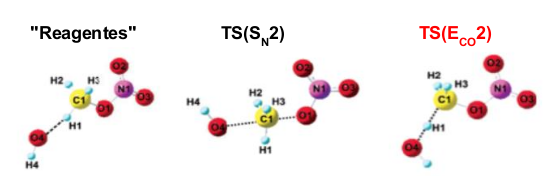
\includegraphics[width=.8\linewidth]{fig/estadosTQ3}
\end{figure}

\textbf{a)} Considerando que a intensidade relativa pode ser considerada como proporcional a concentração dos reagentes, escreva as derivadas \(\frac{d \ce{[HO^-]}}{dt}\), \(\frac{d \ce{[NO3^-]}}{dt}\), \( \frac{ \ce{[NO2^-]}}{dt}\) em função das constantes de velocidades e das concentrações das espécies envolvidas.

\textbf{b)} Com os dados cinéticos do gráfico (também apresentados na tabela no fim dessa questão), obtenha a constante de decaimento de \ce{^-OH} experimental, os valores de \ce{k_{SN 2}} e \ce{k_Eco 2}.

\textbf{c)} Mostre a partir das derivadas parciais que o valor da constante de decaimento de \ce{^-OH} experimental, os valores de \ce{k_{SN 2}} e \ce{k_{Eco 2}}.

A equação de Eyring relaciona o valor da constante de velocidade com a energia livre de ativação, que pode ser representada pela entalpia e entropia de ativação conforme a seguinte equação:

\begin{align*}
    k(T) = \frac{k_b T}{h} e^{\frac{\Delta S^\ddagger}{R}} e^{-\frac{\Delta H^\ddagger}{RT}}   
\end{align*}

\textbf{d)} Considerando que a energia de interação dos estados de transição é praticamente a mesma, dada a precisão dos cálculos teóricos utilizados, explique porque a reação \ce{Eco 2}é mais rápida do que a \ce{SN 2}.

\textbf{e)} Com esses dados, é possível afirmar alguma coisa a respeito do papel do nitrato de metila no mecanismo da reação?

Dados cinéticos:

\begin{center}
\begin{tabular}{c c c c}
\toprule
\textbf{tempo/ms} & \textbf{\ce{HO^-}} & \textbf{\ce{NO2^-}} & \textbf{\ce{NO3^-}} \\
\midrule
0   & 0,93 & 0,08 & 0,00 \\
50  & 0,71 & 0,29 & 0,04 \\
100 & 0,48 & 0,45 & 0,07 \\
150 & 0,35 & 0,57 & 0,09 \\
200 & 0,24 & 0,65 & 0,10 \\
250 & 0,18 & 0,72 & 0,12 \\
300 & 0,12 & 0,76 & 0,12 \\
350 & 0,10 & 0,79 & 0,13 \\
400 & 0,07 & 0,80 & 0,13 \\
450 & 0,06 & 0,83 & 0,13 \\
500 & 0,04 & 0,83 & 0,14 \\
550 & 0,03 & 0,83 & 0,13 \\
600 & 0,03 & 0,84 & 0,13 \\
650 & 0,02 & 0,84 & 0,14 \\
700 & 0,02 & 0,85 & 0,14 \\
750 & 0,02 & 0,85 & 0,14 \\
800 & 0,01 & 0,86 & 0,14 \\
\bottomrule
\end{tabular}
\end{center}
